\section{Experiments}
\label{sec:experiments}

We evaluate the two levels of RAL-MoE-ROM through complementary benchmark roles.
All three two-dimensional incompressible-flow datasets span steady, Hopf-onset,
and periodic dynamics as the Reynolds number varies. The circular-cylinder
benchmark provides the local-specialist ablation, the centered-square benchmark
provides matched $S$--$H$ and $H$--$P$ routing/fusion comparisons, and the
fluidic-pinball benchmark provides the autonomous comparison with a classical
POD--Galerkin baseline. Table~\ref{tab:benchmark_summary} summarizes this scope.
All training, validation, and test partitions are defined by complete parameter
trajectories; chart-wise ranges and split counts are reported in
Appendix~\ref{app:implementation}.

Errors $E_u$ and $E_p$ are relative physical-field errors in percent, aggregated
according to each benchmark's evaluation protocol; $E_{\mathrm{joint}}=E_u+E_p$.
The sum of displayed component errors can differ slightly from the reported
joint error because values are rounded independently.
``Divergent'' denotes an evaluation window that violates the predefined
rollout-divergence criterion, including non-finite states or threshold
violations. N/E denotes not evaluable under the prescribed rollout criterion;
table-specific notes give the reason.

\begin{table}[t]
\centering
\caption{Experimental scope and primary benchmark roles. Local ranks list
$(r_u,r_p)_S$, $(r_u,r_p)_H$, and $(r_u,r_p)_P$, in that order; horizons give
$K_S/K_H/K_P$. Here $K$ counts evaluation rollout steps at the corresponding
sampling interval. Additional overlap and periodic-core settings are identified
in the corresponding comparisons.}
\label{tab:benchmark_summary}
\small
\setlength{\tabcolsep}{4pt}
\begin{tabular}{@{}>{\raggedright\arraybackslash}p{2.15cm}
>{\raggedright\arraybackslash}p{1.30cm}
>{\raggedright\arraybackslash}p{4.05cm}
>{\raggedright\arraybackslash}p{1.80cm}
>{\raggedright\arraybackslash}p{2.50cm}@{}}
\toprule
Benchmark & $Re$ range & Local ranks ($S,H,P$) & Main horizons & Primary role \\
\midrule
Circular cylinder & 20--200 & $(32,32),\ (32,32),\ (32,32)$ & $56/56/48$ & Local specialist ablation \\
\addlinespace
Centered square & 50--150 & $(5,4),\ (11,11),\ (28,26)$ & $16/48/24$ & Routing and fusion \\
\addlinespace
Fluidic pinball & 10--60 & $(4,3),\ (5,5),\ (17,16)$ & $56/56/32$ & Autonomous baseline \\
\bottomrule
\end{tabular}
\end{table}

\subsection{Do local specialists support long autonomous rollouts?}

The learned fluidic-pinball specialists complete all four evaluation settings
without divergent windows, whereas POD--Galerkin fails in every steady window
and in part of the Hopf evaluation (Table~\ref{tab:pinball_autonomous}).
The Hopf baseline has a joint error of $48.94\%$ on finite windows, compared
with $2.085\%$ for RAL-MoE-ROM; at periodic $K=32$, the joint error decreases
from $43.20\%$ to $0.8415\%$. The separate velocity and pressure columns
show the particularly large pressure discrepancy of the projected baseline.
These results support autonomous prediction over the evaluated horizons.
The circular-cylinder ablation and centered-square local-specialist results
provide complementary evidence in Table~\ref{tab:compact_ablation} and
Appendix~\ref{app:square}, respectively.

\begin{table}[t]
\centering
\caption{Autonomous local-specialist prediction on the fluidic-pinball benchmark.
Errors are percentages; lower is better. Periodic core is a second evaluation setting
within the periodic regime.}
\label{tab:pinball_autonomous}
\small
\setlength{\tabcolsep}{5pt}
\begin{threeparttable}
\begin{tabular}{@{}llrrr@{}}
\toprule
Evaluation setting & Model & $E_u$ & $E_p$ & $E_{\mathrm{joint}}$ \\
\midrule
Steady ($K=56$) & POD--Galerkin & N/E$^\dagger$ & N/E$^\dagger$ & N/E$^\dagger$ \\
 & RAL-MoE-ROM & 0.2247 & 0.7593 & 0.9840 \\
\addlinespace
Hopf ($K=56$) & POD--Galerkin & 0.4378$^\ddagger$ & 48.50$^\ddagger$ & 48.94$^\ddagger$ \\
 & RAL-MoE-ROM & 0.0995 & 1.986 & 2.085 \\
\addlinespace
Periodic ($K=32$) & POD--Galerkin & 1.641 & 41.56 & 43.20 \\
 & RAL-MoE-ROM & 0.2897 & 0.5518 & 0.8415 \\
\addlinespace
Periodic core ($K=56$) & POD--Galerkin & 2.555 & 39.36 & 41.91 \\
 & RAL-MoE-ROM & 0.6222 & 1.050 & 1.672 \\
\bottomrule
\end{tabular}
\begin{tablenotes}[flushleft]
\footnotesize
\item[$\dagger$] All 448 evaluation windows violate the predefined rollout-divergence criterion.
\item[$\ddagger$] Errors are computed on finite evaluation windows, including threshold-violating windows; 141 of 320 Hopf windows violate the divergence criterion. All RAL-MoE-ROM settings and both periodic POD--Galerkin settings have zero divergent windows.
\end{tablenotes}
\end{threeparttable}
\end{table}

\subsection{Does learned physical-space fusion improve overlap prediction?}

Having evaluated autonomous local dynamics, we next isolate the second level
of the hierarchy. The centered-square benchmark provides both $S$--$H$ and
$H$--$P$ overlaps under a common $K=24$ protocol and is therefore the primary
routing/fusion comparison. Table~\ref{tab:routing_fusion} reports joint field
error; separate velocity and pressure errors are given in
Table~\ref{tab:square_fusion_full} in Appendix~\ref{app:square}.

T2-C improves both hard routing and the best fixed individual specialist in
the two tested overlaps. In $H$--$P$, joint error decreases from $1.2079\%$
for the best single specialist and $1.8473\%$ for E2 Top-1 to $0.8465\%$.
Its proximity to the convex oracle suggests that the learned correction
captures most of the available complementarity within the tested convex
fusion class. Figure~\ref{fig:square_overlap} shows representative physical
fields and velocity-error maps; parameter-wise results and the fluidic-pinball
overlap study appear in Appendices~\ref{app:square} and \ref{app:pinball}.

\begin{table}[t]
\centering
\caption{Cross-regime routing and fusion on the centered-square benchmark at
$K=24$. Entries are $E_{\mathrm{joint}}$ (\%); lower is better. Best single
is the lowest-error fixed specialist over each overlap's evaluation set
(Hopf for $S$--$H$, Periodic for $H$--$P$), not a window-wise selection.
The convex oracle is an a posteriori reference unavailable during prediction;
bold marks the best deployable assembly.}
\label{tab:routing_fusion}
\small
\setlength{\tabcolsep}{5pt}
\begin{tabular}{@{}lrrrrrr@{}}
\toprule
Overlap & Best single & E2 Top-1 & Equal & E2 prob. & T2-C & Oracle \\
\midrule
$S$--$H$ & 1.7298 & 1.7298 & 3.0321 & 2.1847 & \textbf{1.1958} & 1.1842 \\
$H$--$P$ & 1.2079 & 1.8473 & 1.6146 & 1.6618 & \textbf{0.8465} & 0.8384 \\
\bottomrule
\end{tabular}
\end{table}

\begin{figure}[t]
\centering
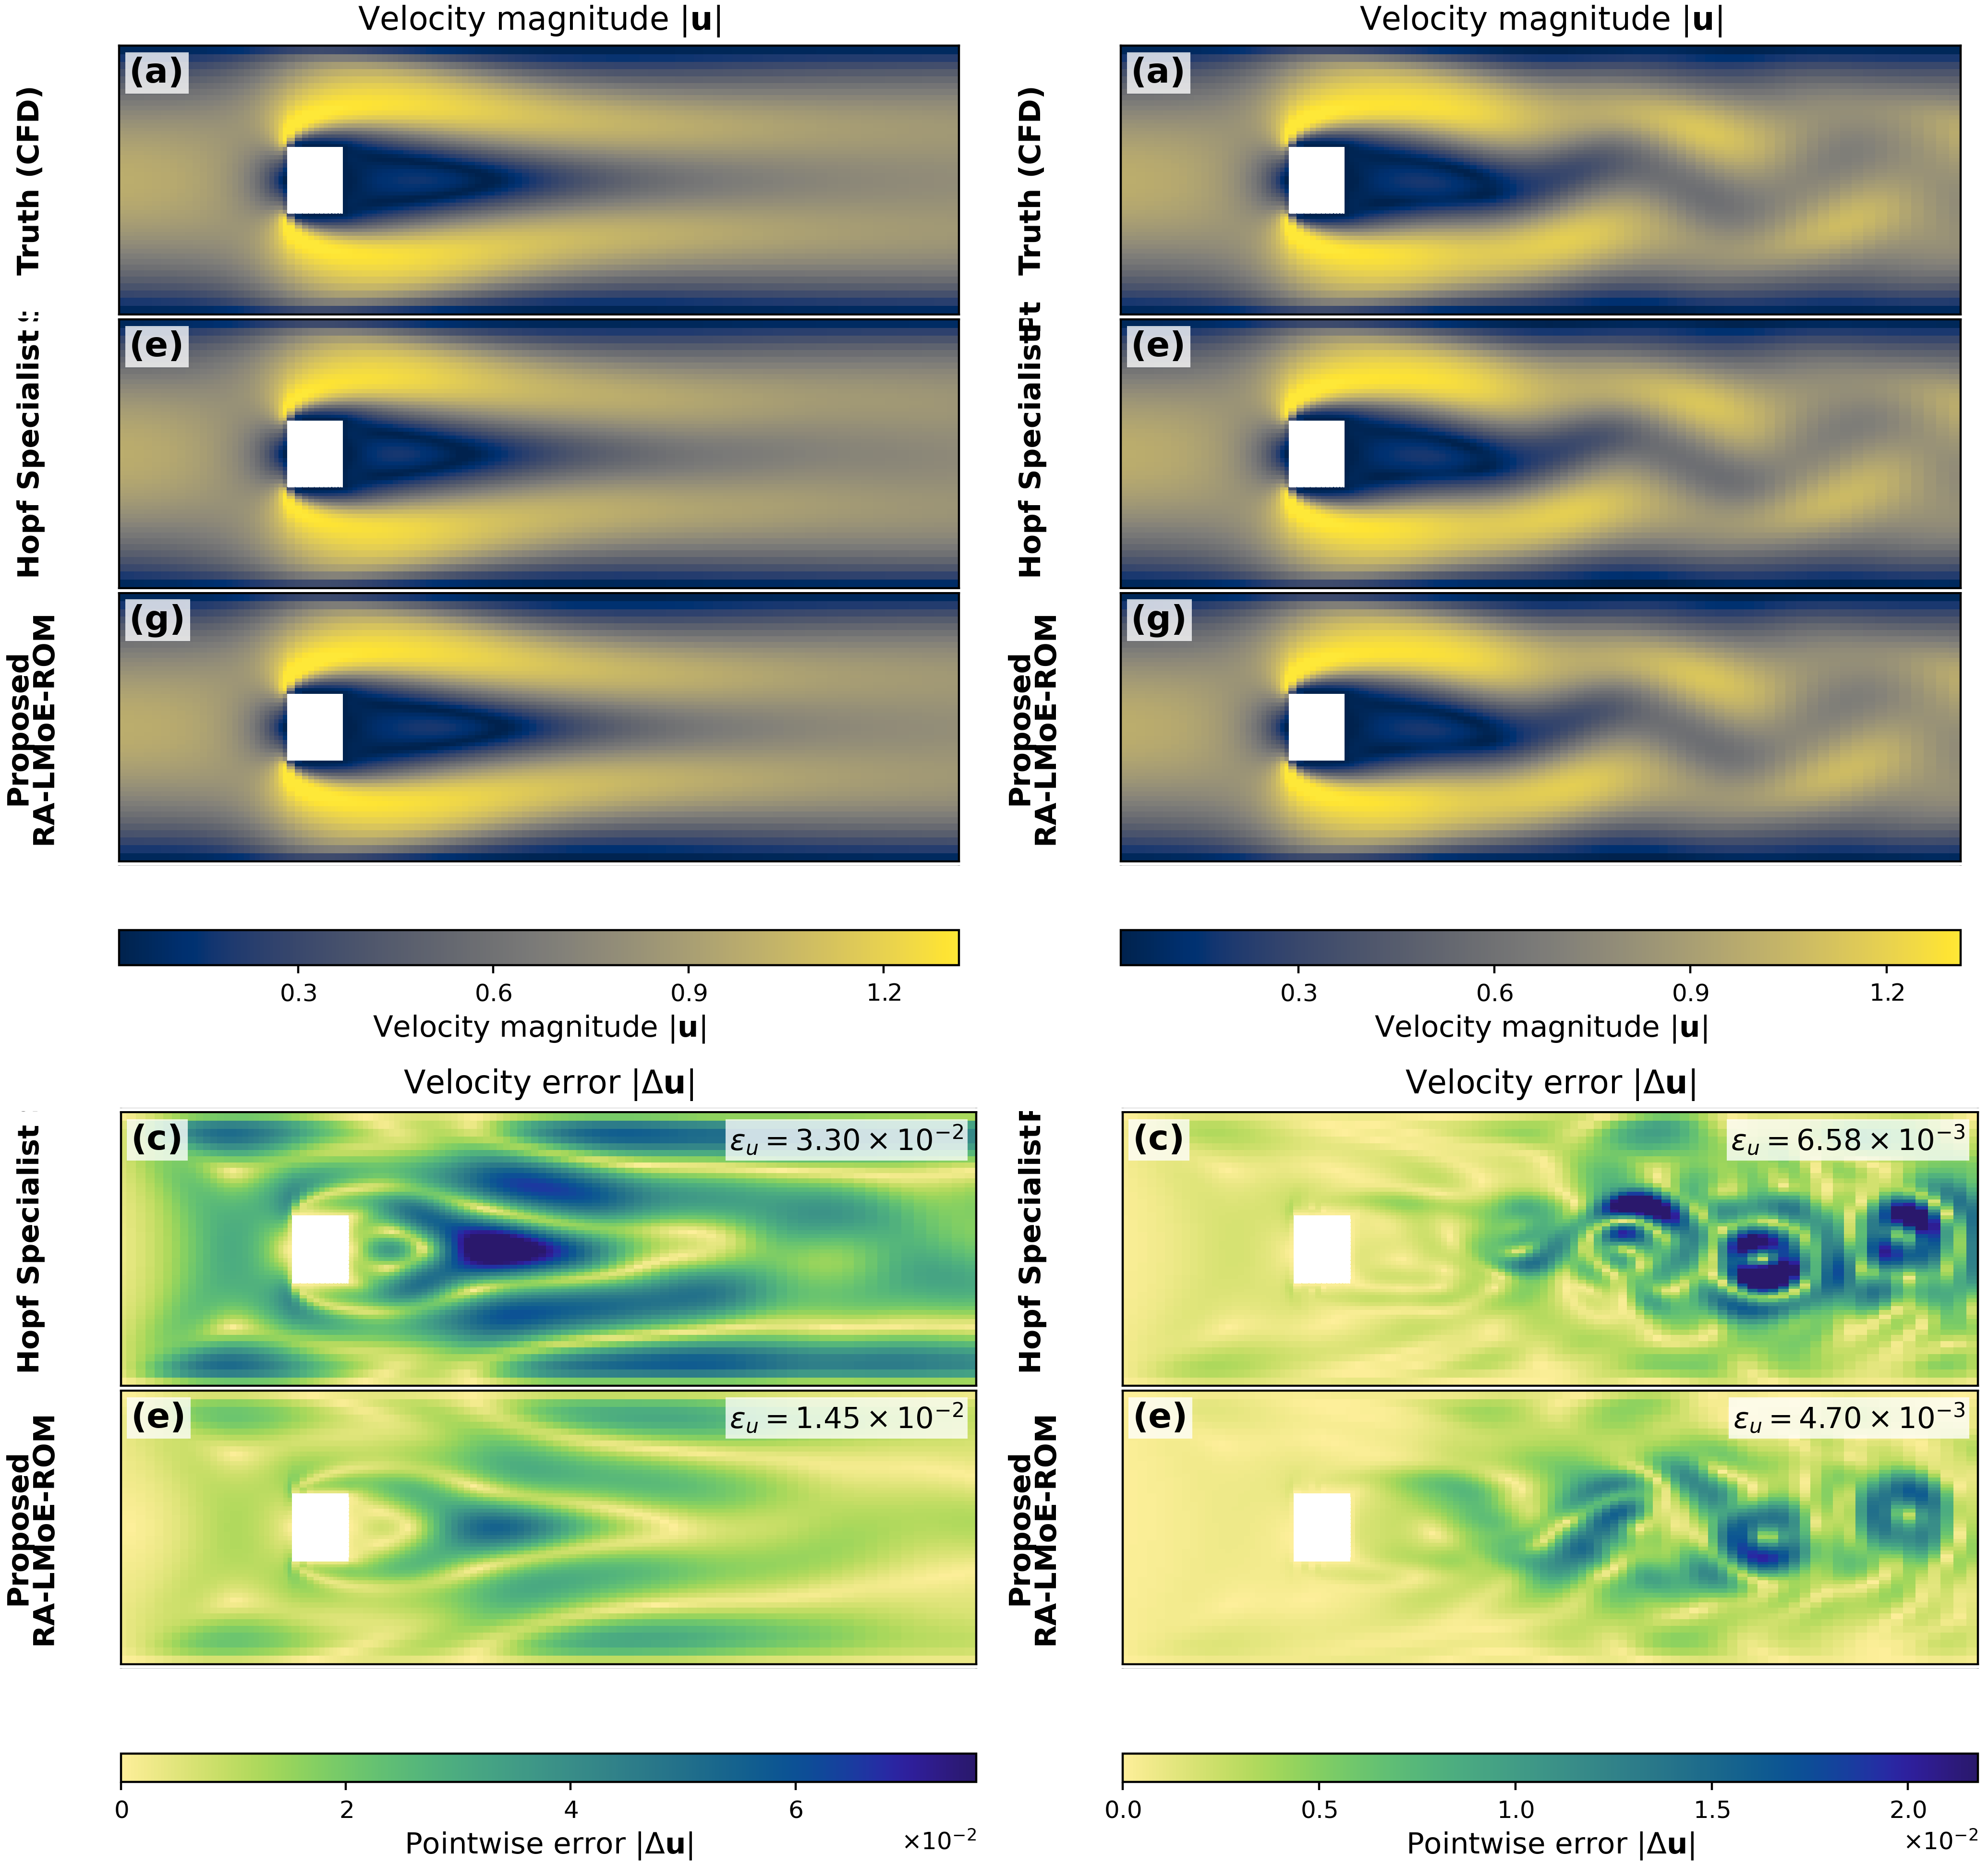
\includegraphics[width=\linewidth]{figures/square_overlap_compact.png}
\caption{Representative cross-regime predictions on the centered-square benchmark. The left and right panels correspond to the $S$--$H$ and $H$--$P$ overlaps, respectively. T2-C combines independently evolved specialists after physical reconstruction and reduces the velocity-field discrepancy relative to the corresponding single-specialist prediction. Complete velocity and pressure fields are reported in Appendix~\ref{app:square}.}
\label{fig:square_overlap}
\end{figure}

\subsection{What do local architectural components contribute?}

The circular-cylinder comparison isolates three local modeling choices
(Table~\ref{tab:compact_ablation}). Vanilla-FNN-MoE replaces the structured
expert map with conventional feed-forward experts, DataOnly-MoE removes the
projected Galerkin and Pressure--Poisson contributions, and Global MoE replaces
the local charts and specialists with one global model. The comparison uses
physical-field errors so that models with different reduced coordinates can
be evaluated on a common quantity.

\begin{table}[t]
\centering
\caption{Local architecture ablation on the circular-cylinder benchmark.
Each regime cell reports the min--max $E_u$ range (upper line) and $E_p$
range (lower line) over held-out Reynolds-number trajectories, in percent.
These are field-error ranges, not means or uncertainty intervals.
N/E denotes not evaluable under the prescribed rollout criterion: the
Vanilla-FNN-MoE Hopf model does not meet the validation-stage stability
requirement and is not evaluated on held-out trajectories.}
\label{tab:compact_ablation}
\small
\setlength{\tabcolsep}{4pt}
\begin{tabular}{@{}lccc@{}}
\toprule
Model & Steady ($K=56$) & Hopf ($K=56$) & Periodic ($K=48$) \\
\midrule
RAL-MoE-ROM
& \shortstack{0.0330--0.1723\\0.2500--1.3249}
& \shortstack{0.0032--0.0288\\0.0355--0.4321}
& \shortstack{0.3809--1.3473\\1.6825--5.9601} \\
\addlinespace
Vanilla-FNN-MoE
& \shortstack{0.0384--0.2995\\2.2163--18.5603}
& N/E
& \shortstack{1.0393--3.0836\\3.9659--13.3257} \\
\addlinespace
DataOnly-MoE
& \shortstack{0.1637--0.5122\\4751.1025--27275.4645}
& \shortstack{0.1260--0.3880\\1280.2811--1524.5949}
& \shortstack{0.7854--1.8677\\2.2511--10.8189} \\
\addlinespace
Global MoE
& \shortstack{0.0845--0.3404\\1.5226--7.4363}
& \shortstack{0.0110--0.0268\\0.0560--0.2882}
& \shortstack{0.5873--1.1726\\2.1896--6.3566} \\
\bottomrule
\end{tabular}
\end{table}

Structured specialists improve the steady and periodic error ranges over
Vanilla-FNN-MoE, which does not meet the validation-stage stability requirement
for the Hopf evaluation. For example,
the steady pressure range is $0.2500$--$1.3249\%$ for RAL-MoE-ROM versus
$2.2163$--$18.5603\%$ for Vanilla-FNN-MoE. Removing the physical backbone
particularly degrades steady and Hopf pressure prediction. The global model
remains competitive in Hopf and periodic physical-field errors, so
localization is not uniformly superior; its role is to provide regime-specific
coordinates and dynamics that can participate in cross-regime assembly.
The local comparisons address expert structure, physics, and localization,
while Table~\ref{tab:routing_fusion} separately evaluates the outer assembly.
